\newpage
\section{Okno działki}

\begin{table}[H]
    \begin{center}
    \label{tab:table}
    \begin{tabularx}{1.1\textwidth} { 
    >{\raggedright\arraybackslash}X 
    | >{\raggedright\arraybackslash}X 
    | >{\raggedleft\arraybackslash}X}
    \textbf{Funkcja} & \textbf{Opis} & \textbf{Priorytet}\\
    \hline
    Dodaj obiekt&Pozwala nam dodać obiekt na działce - uruchamia painta (java paint)&H\\
    \hline
    Lista obiektów&Lista zawierająca obiekty na działce, docelowo może zawierać pod listy podzielone kategoriami&H\\
    \hline
    Wybór&Pozwala nam wybrać obiekt. Otwiera menu wyboru 4 rzeczyDocelowo na dwa sposoby: &H\\
    &\begin{itemize}
    \item klikając obiekt na mapie tworzymy widok
  	\item wybierając z listy obiektów
	\end{itemize}&\\
	\hline
    Wybierz wiele&Podopcja Listy. Pozwala na wybór wielu obiektów i łączenie ich w grupy&L\\
    \hline
    Powrót do menu&Wraca do home page&H\\
    \hline
    Widok satelitarny&Wraca do home page&L\\
    \hline
    Zdjęcie działki&Pozwala dodać zdjęcie działki wyświetlane w menu&L\\
    \hline

    \end{tabularx}
    \end{center}
    \end{table}
    \begin{figure}[htp]
      \centering
      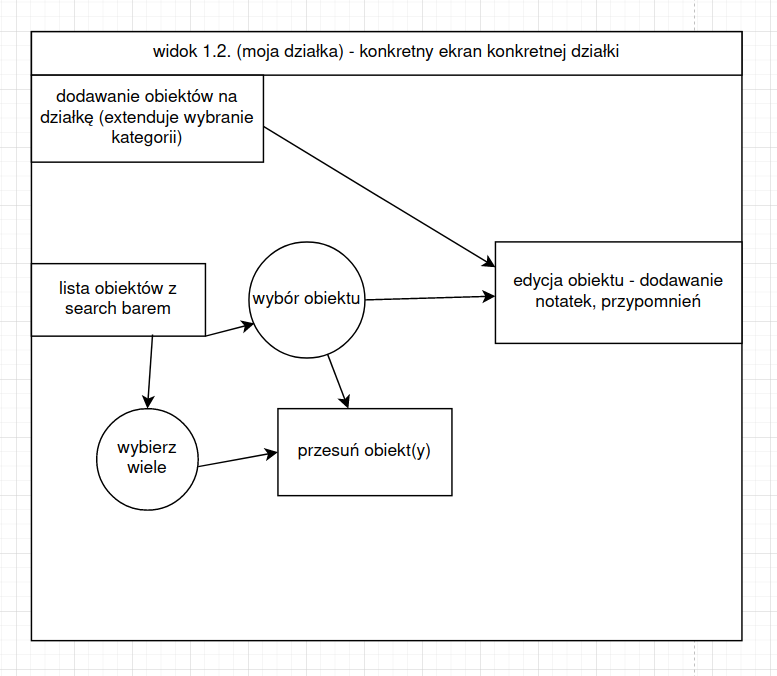
\includegraphics[width=15cm]{ciba10.png}
  \end{figure}    
  